
\begin{figure}[!htbp]
\begin{center}
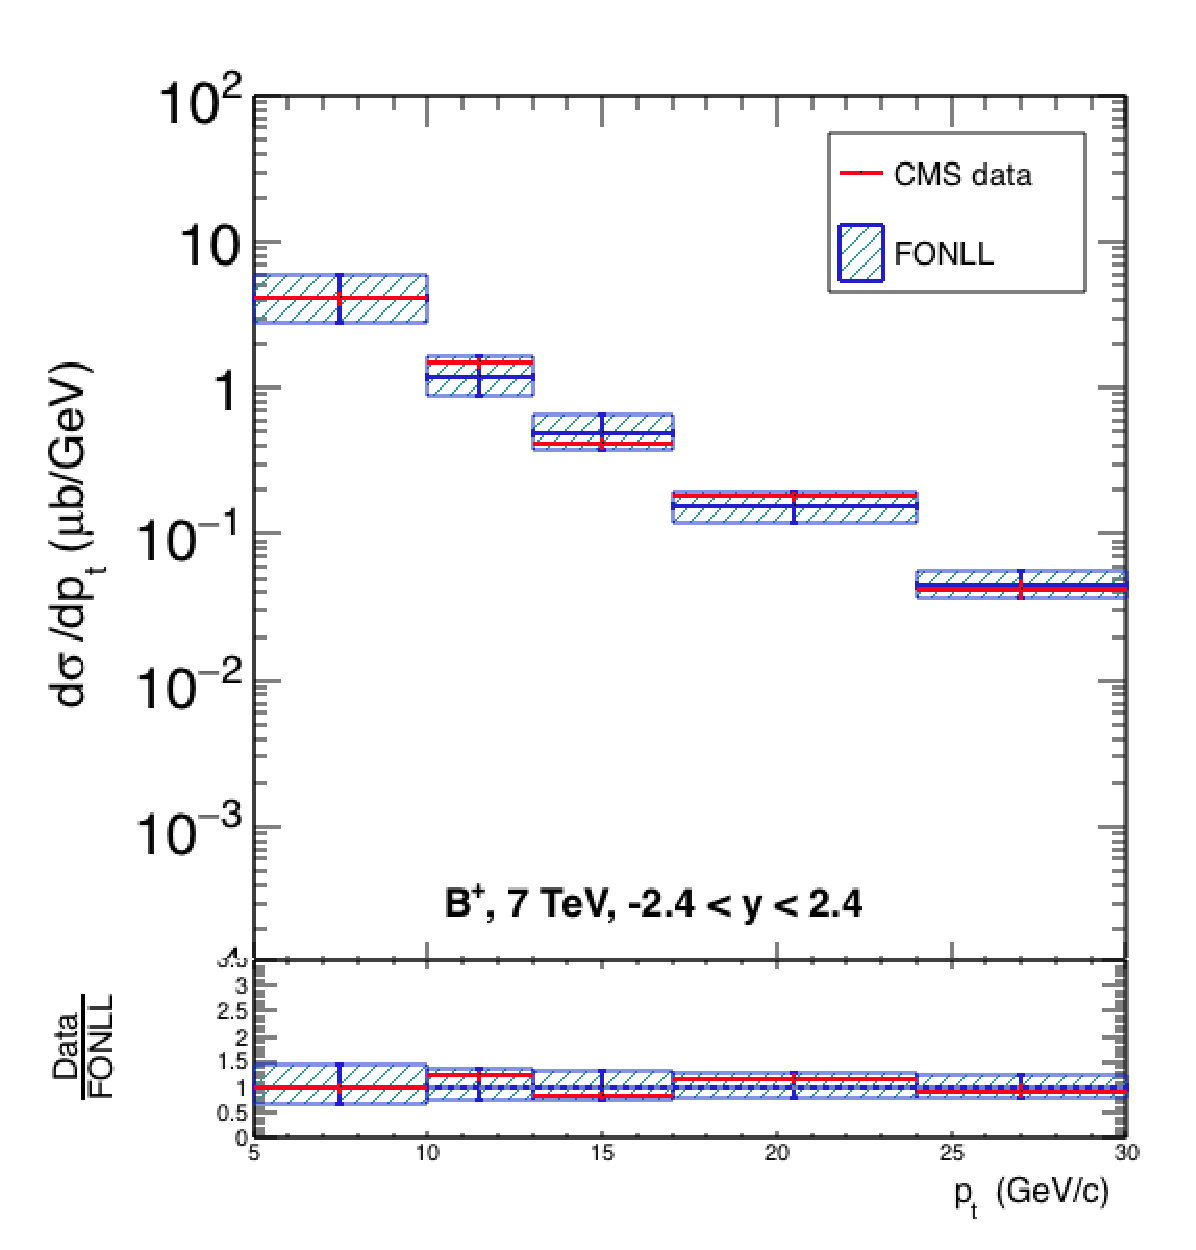
\includegraphics[width=.45\textwidth]{FigCap4/Bplus_7TeV_y_24_24.eps}
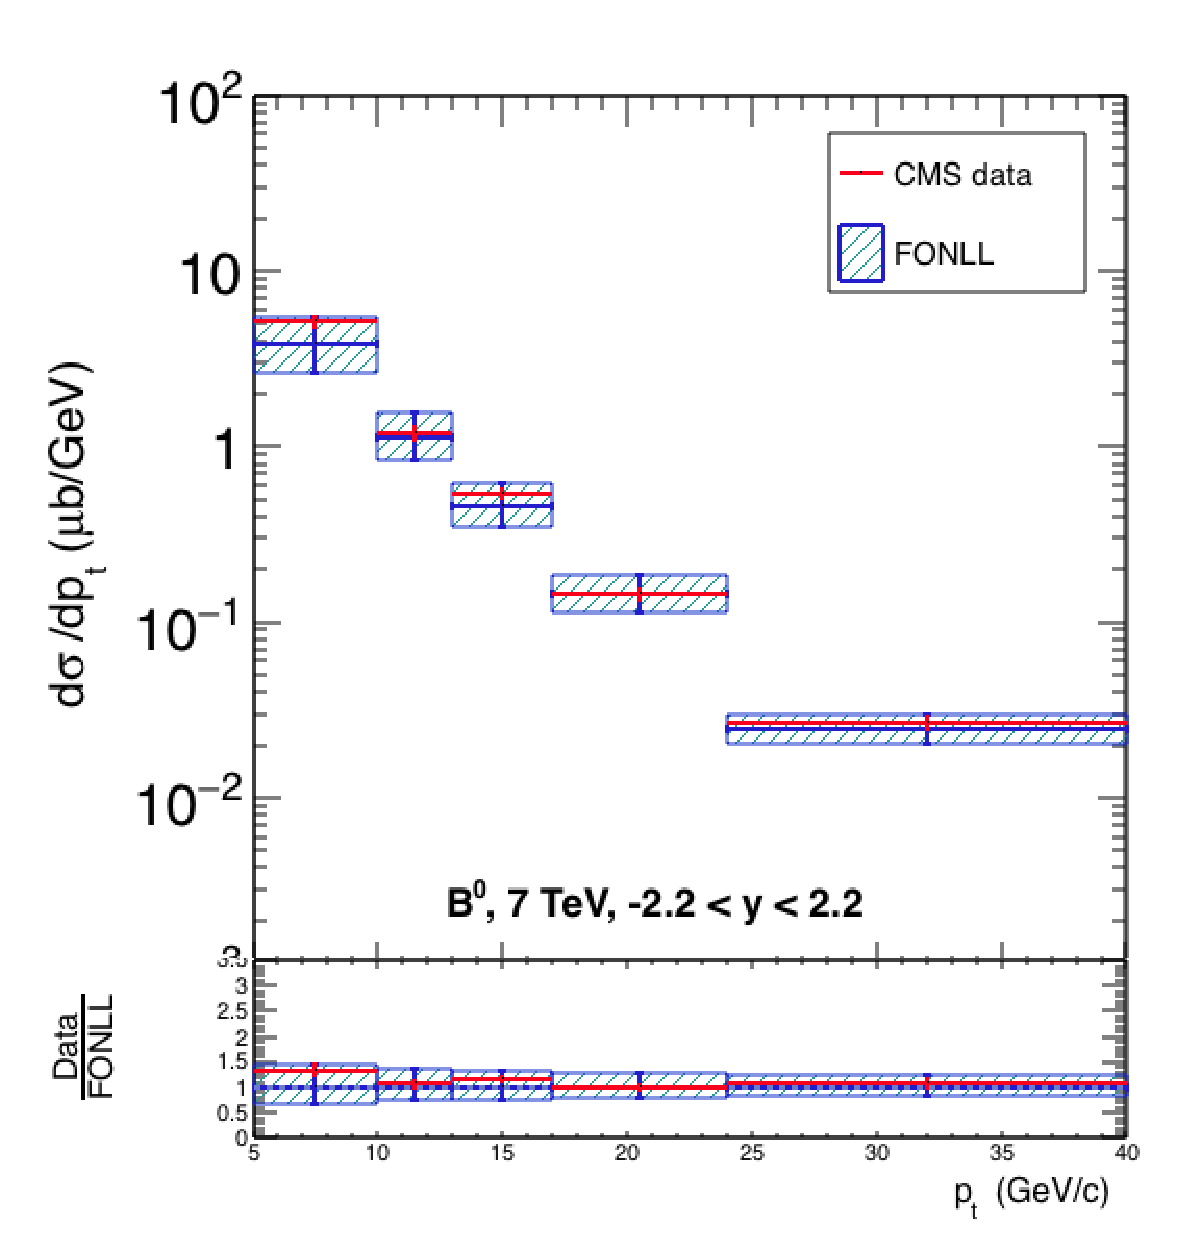
\includegraphics[width=.45\textwidth]{FigCap4/Bzero_7TeV_y_22_22.eps}
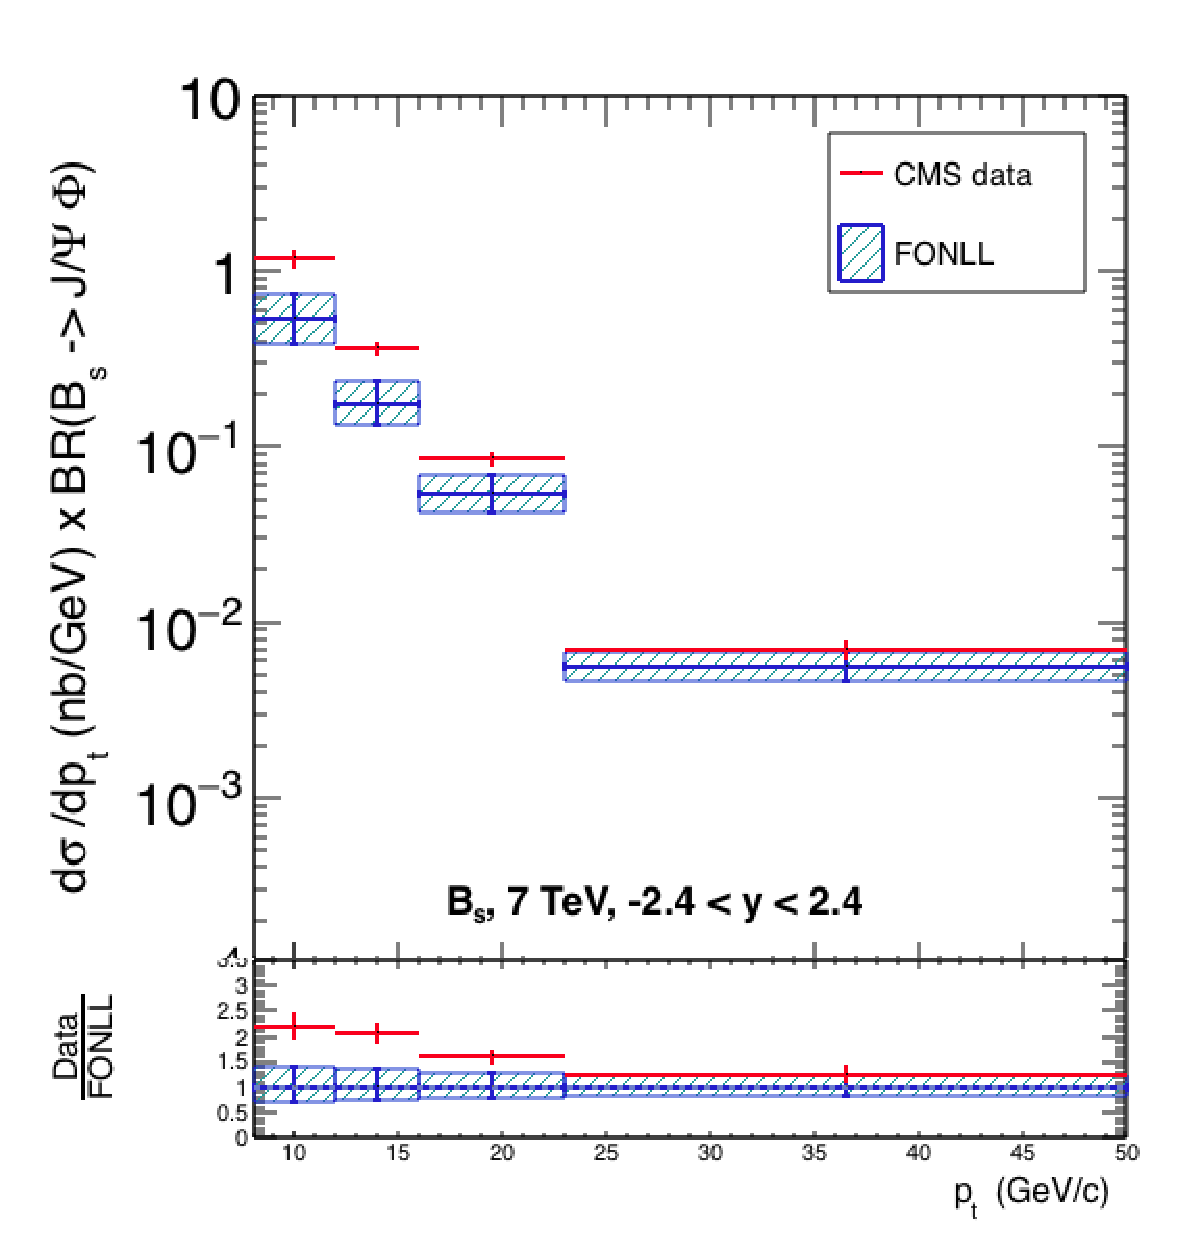
\includegraphics[width=.45\textwidth]{FigCap4/Bs_7TeV_y_24_24.eps}
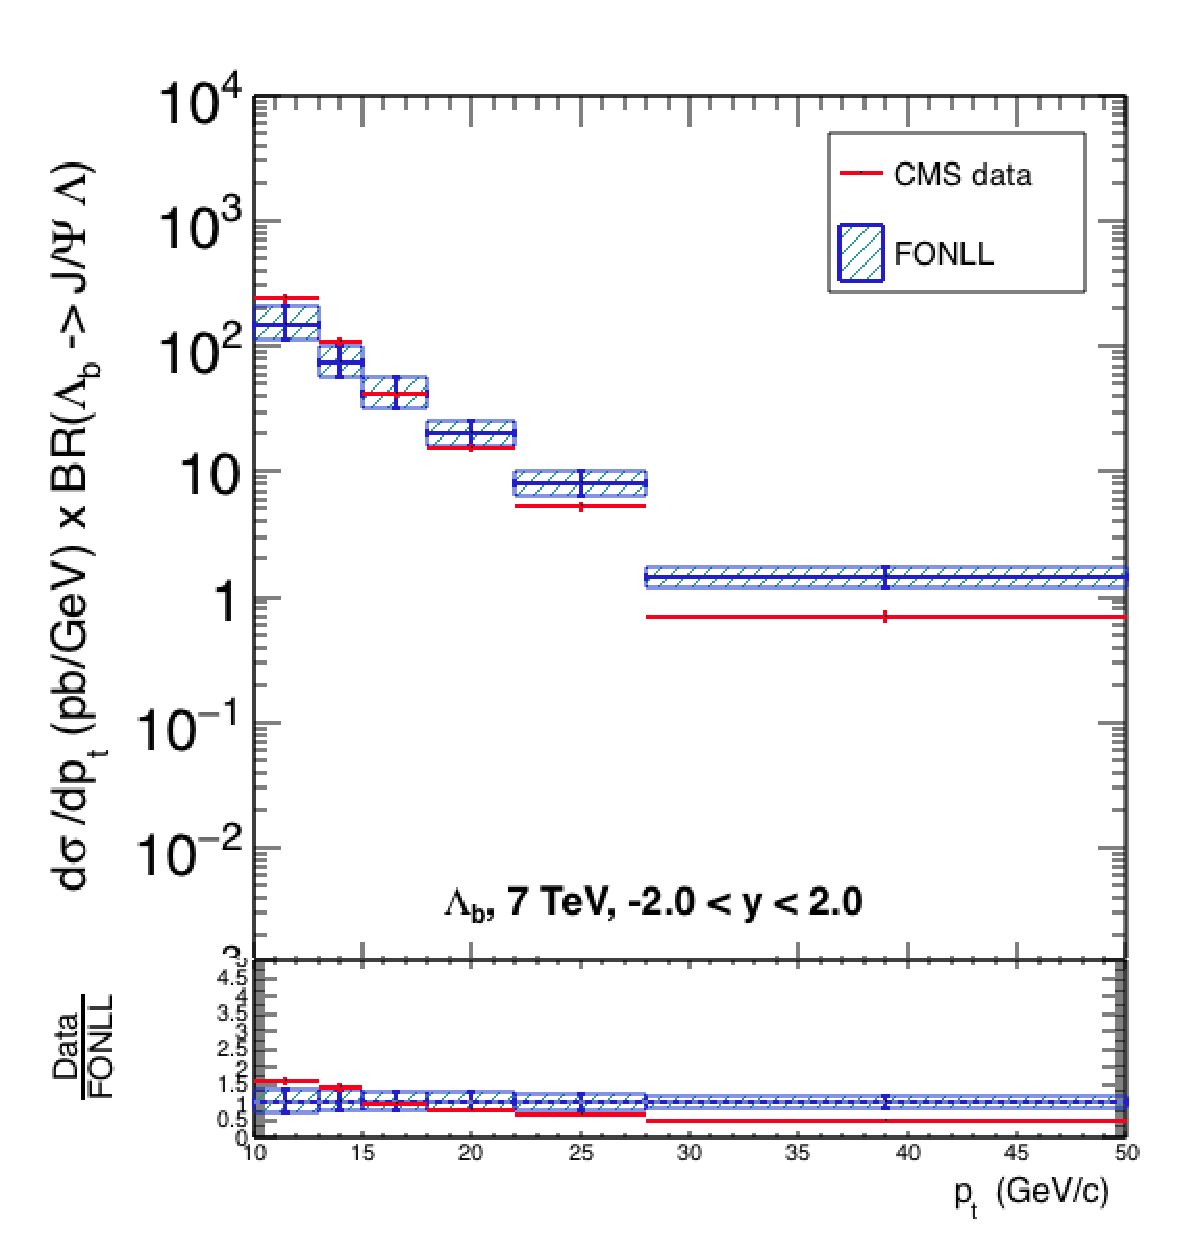
\includegraphics[width=.45\textwidth]{FigCap4/Lambdab_7TeV_y_20_20.eps}
\caption{B$^{+}$, B$^{0}$, B$_{\rm s}$ and $\Lambda_{\rm b}$ differential cross-sections (red points) as a function of $p_{\rm T}$ measured by CMS in pp collisions at 7 TeV at mid-rapidity compared with FONLL predictions at the same energy (blue boxes). }
\label{fig:Bmesons}
\end{center}
\end{figure}

\begin{figure}[!htbp]
\begin{center}
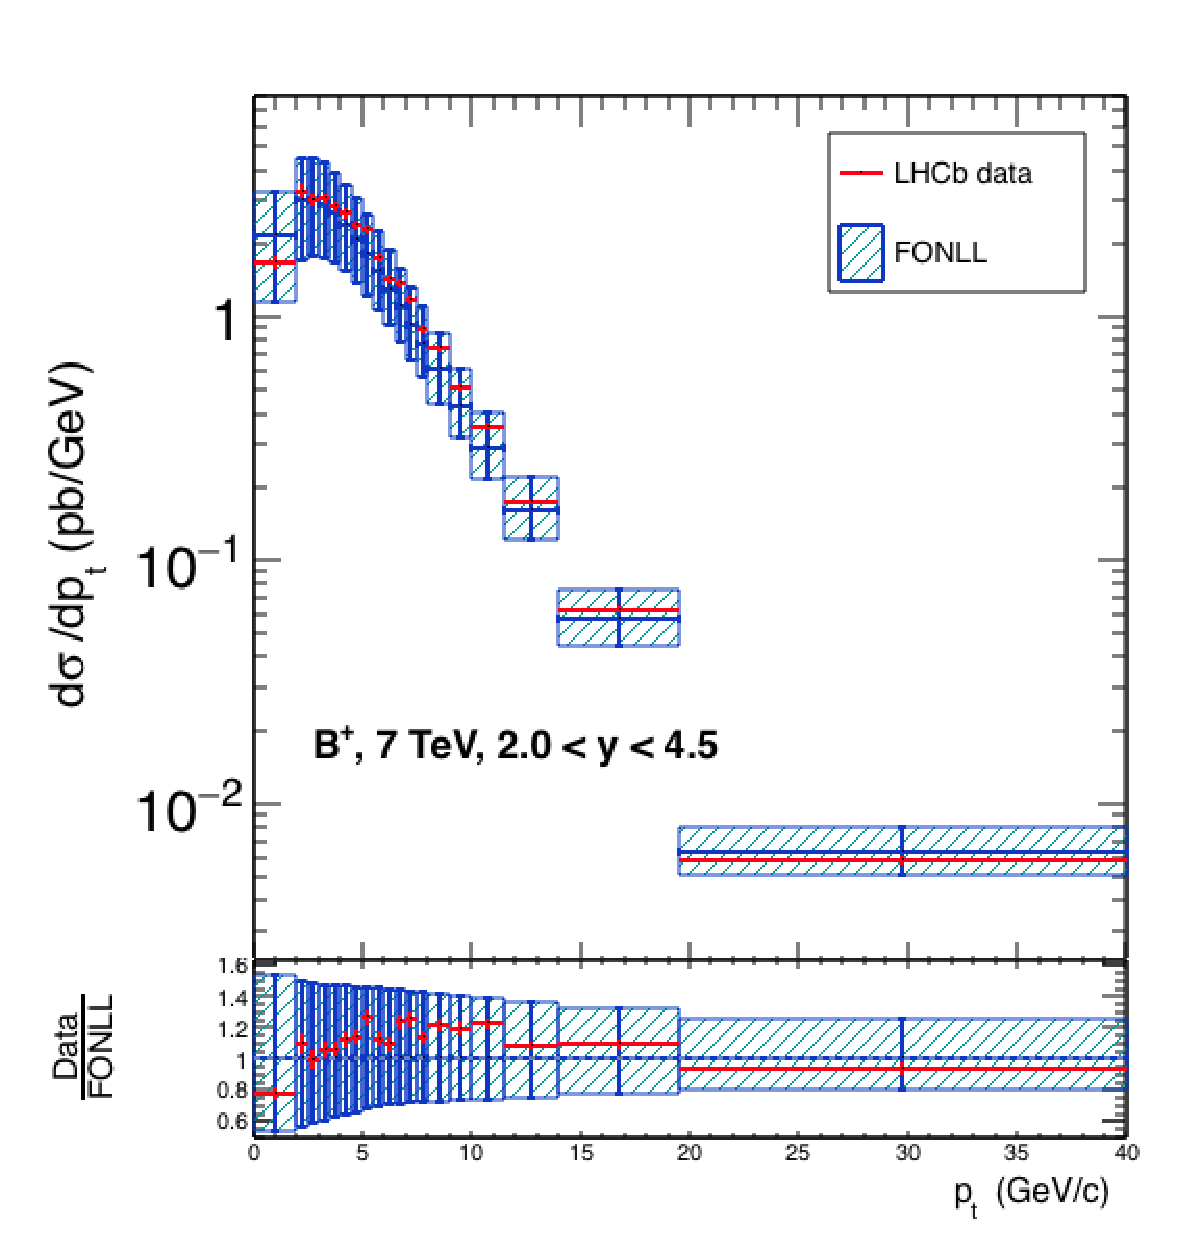
\includegraphics[width=.45\textwidth]{FigCap4/Bplus_7TeV_y_20_45_FF35.eps}
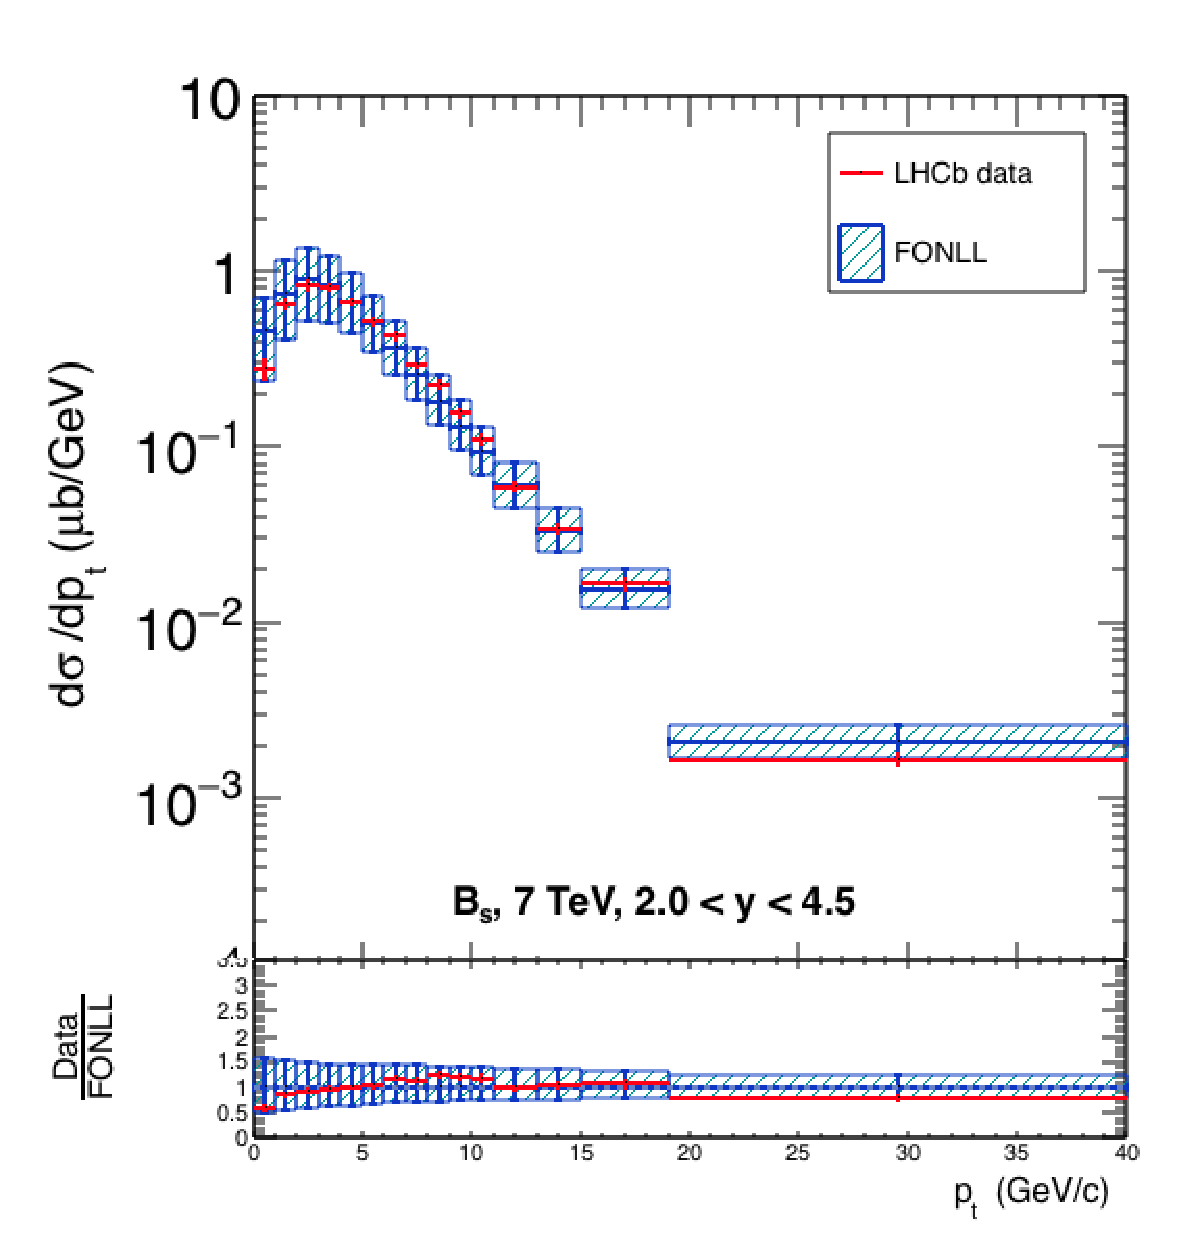
\includegraphics[width=.45\textwidth]{FigCap4/Bs_7TeV_y_20_45.eps}
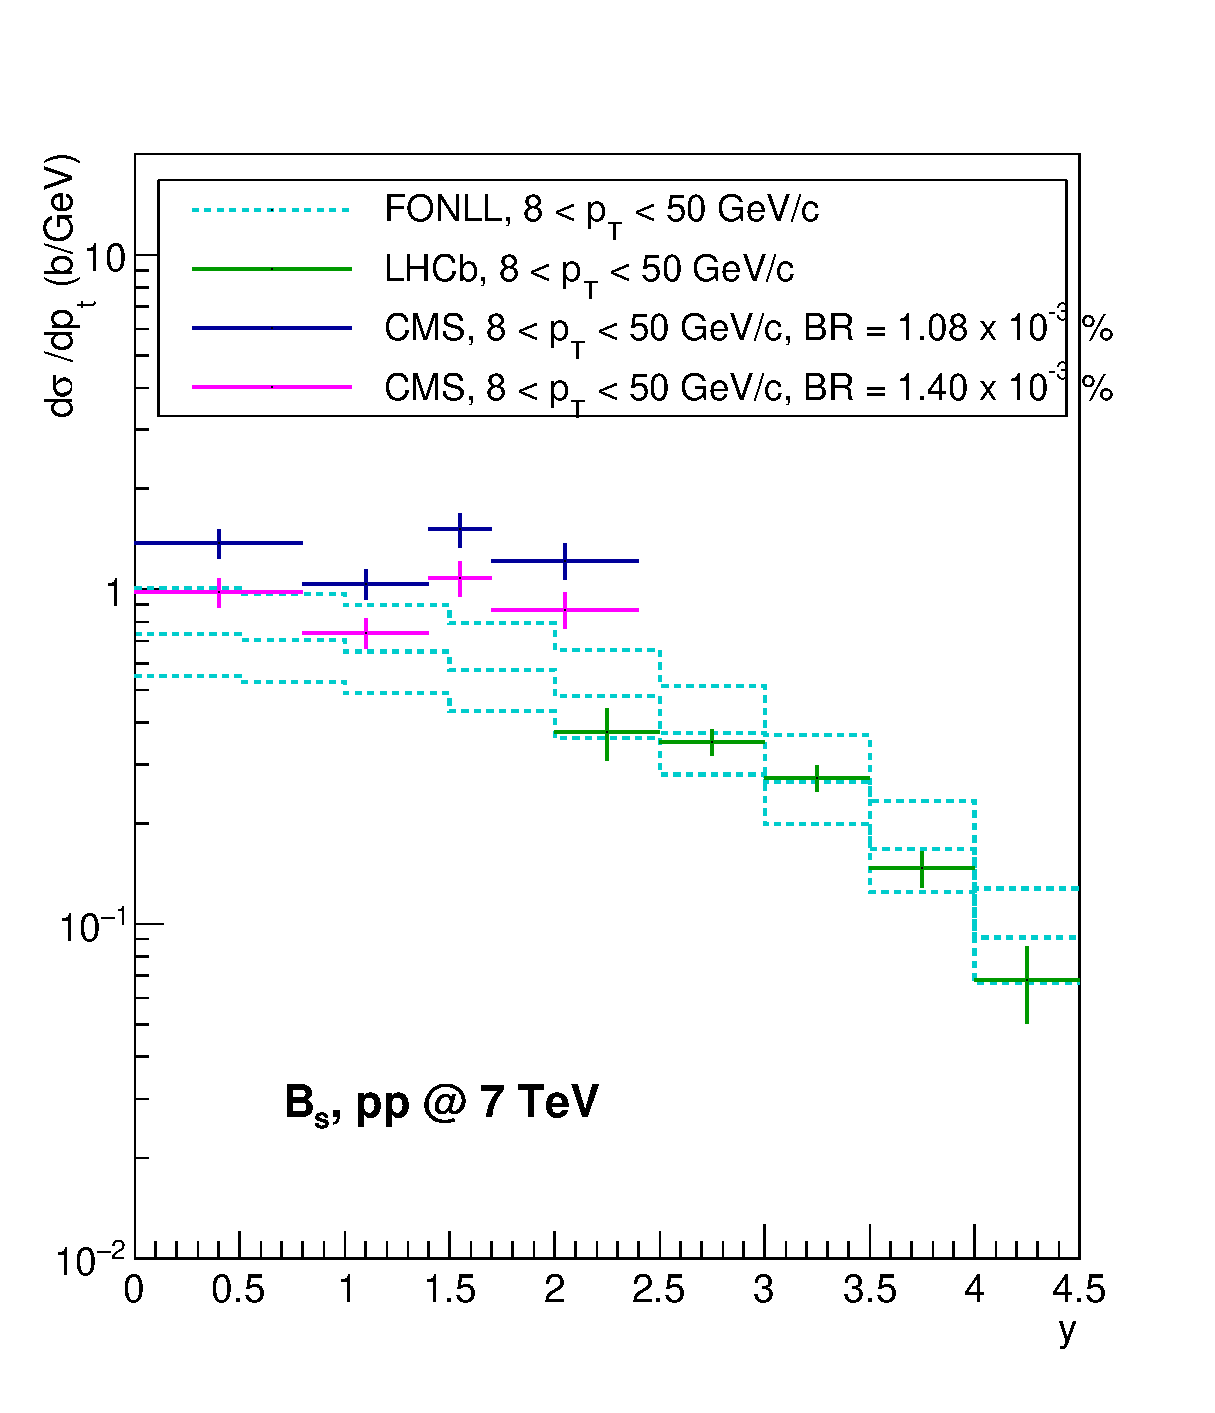
\includegraphics[width=.4\textwidth]{FigCap4/FONLL_CMSvsLHCb_3.eps}
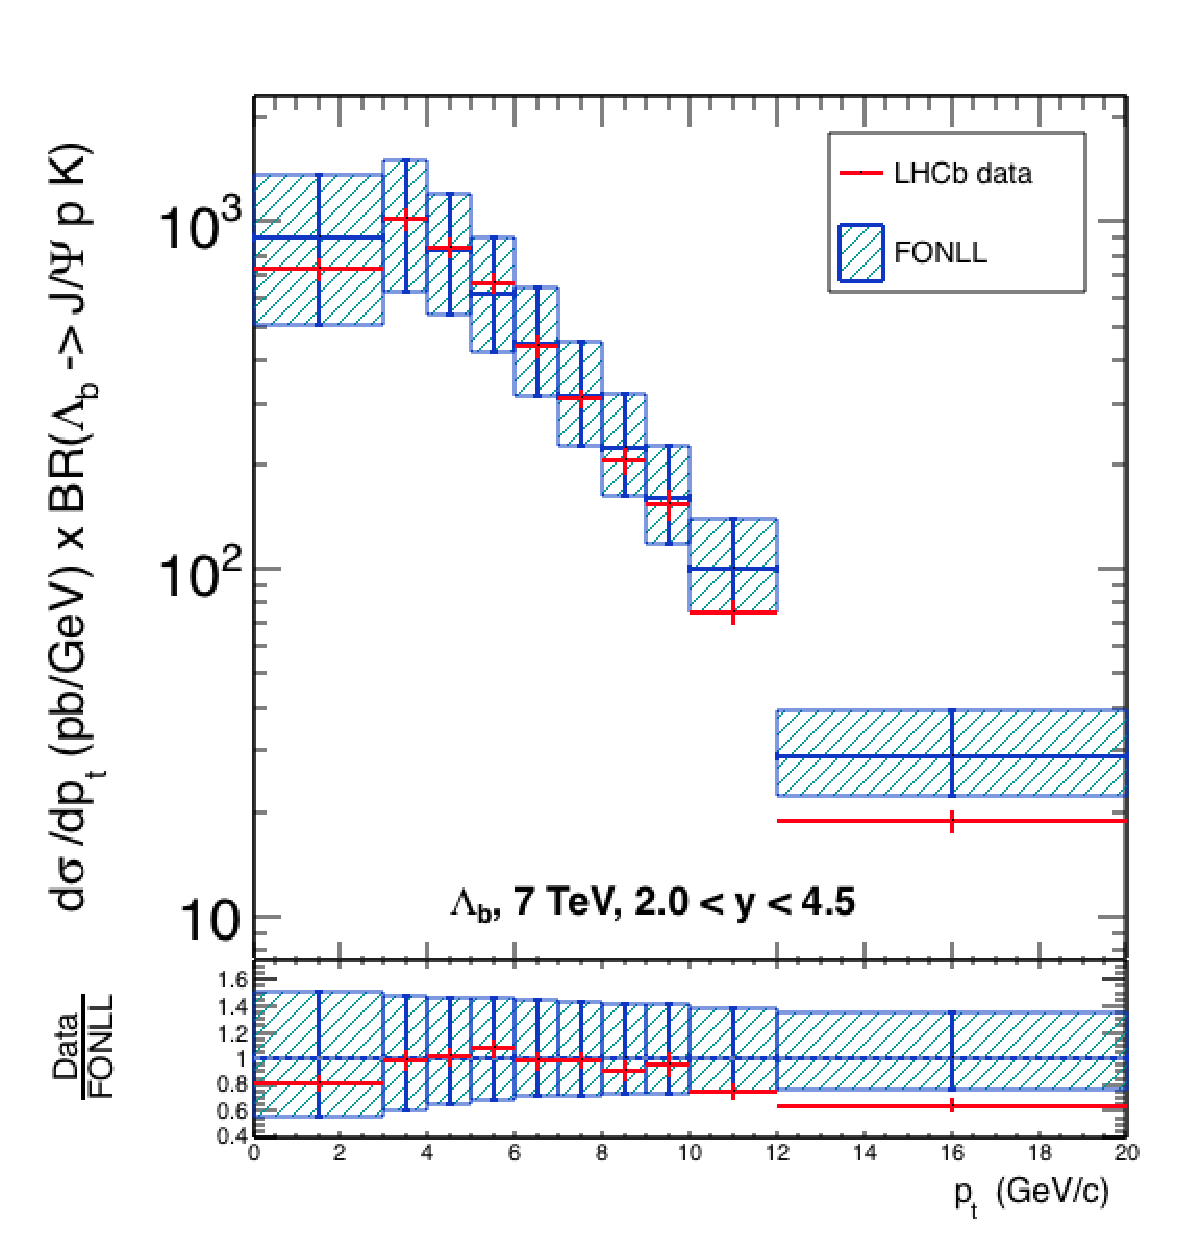
\includegraphics[width=.45\textwidth]{FigCap4/Lambdab_7TeV_y_20_45_FF21_BR6.eps}
\caption{B$^{+}$, B$_{\rm s}$ and $\Lambda_{\rm b}$ differential cross-sections (red points) measured by LHCb in pp collisions at 7 TeV at \mbox{2 $< y_{cm} <$ 4.5} compared with FONLL predictions at the same energy (blue boxes).
In the bottom left plot, B$_{\rm s}$ differential cross-section as a function of $y$ from LHCb is compared to same measurements from CMS at mid-rapidity (8 $< p_{\rm T} <$ 50 GeV/$c$). }
\label{fig:LHCbBmesons}
\end{center}
\end{figure}


\begin{figure}[!htbp]
\begin{center}
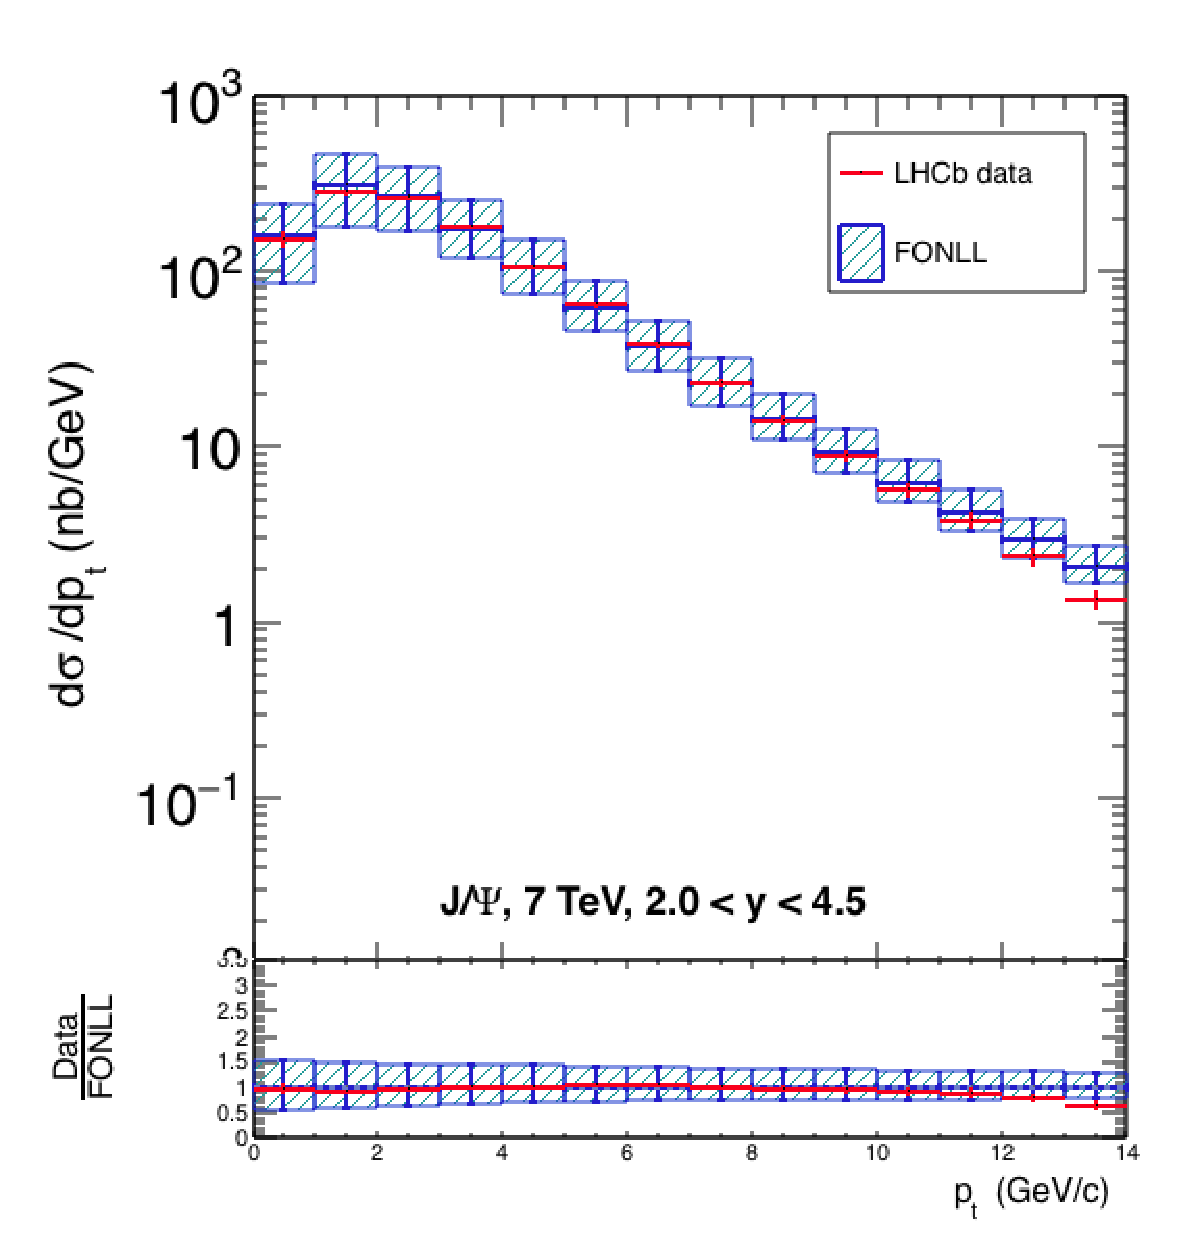
\includegraphics[width=.45\textwidth]{FigCap4/Jpsi_7TeV_y_20_45.eps}
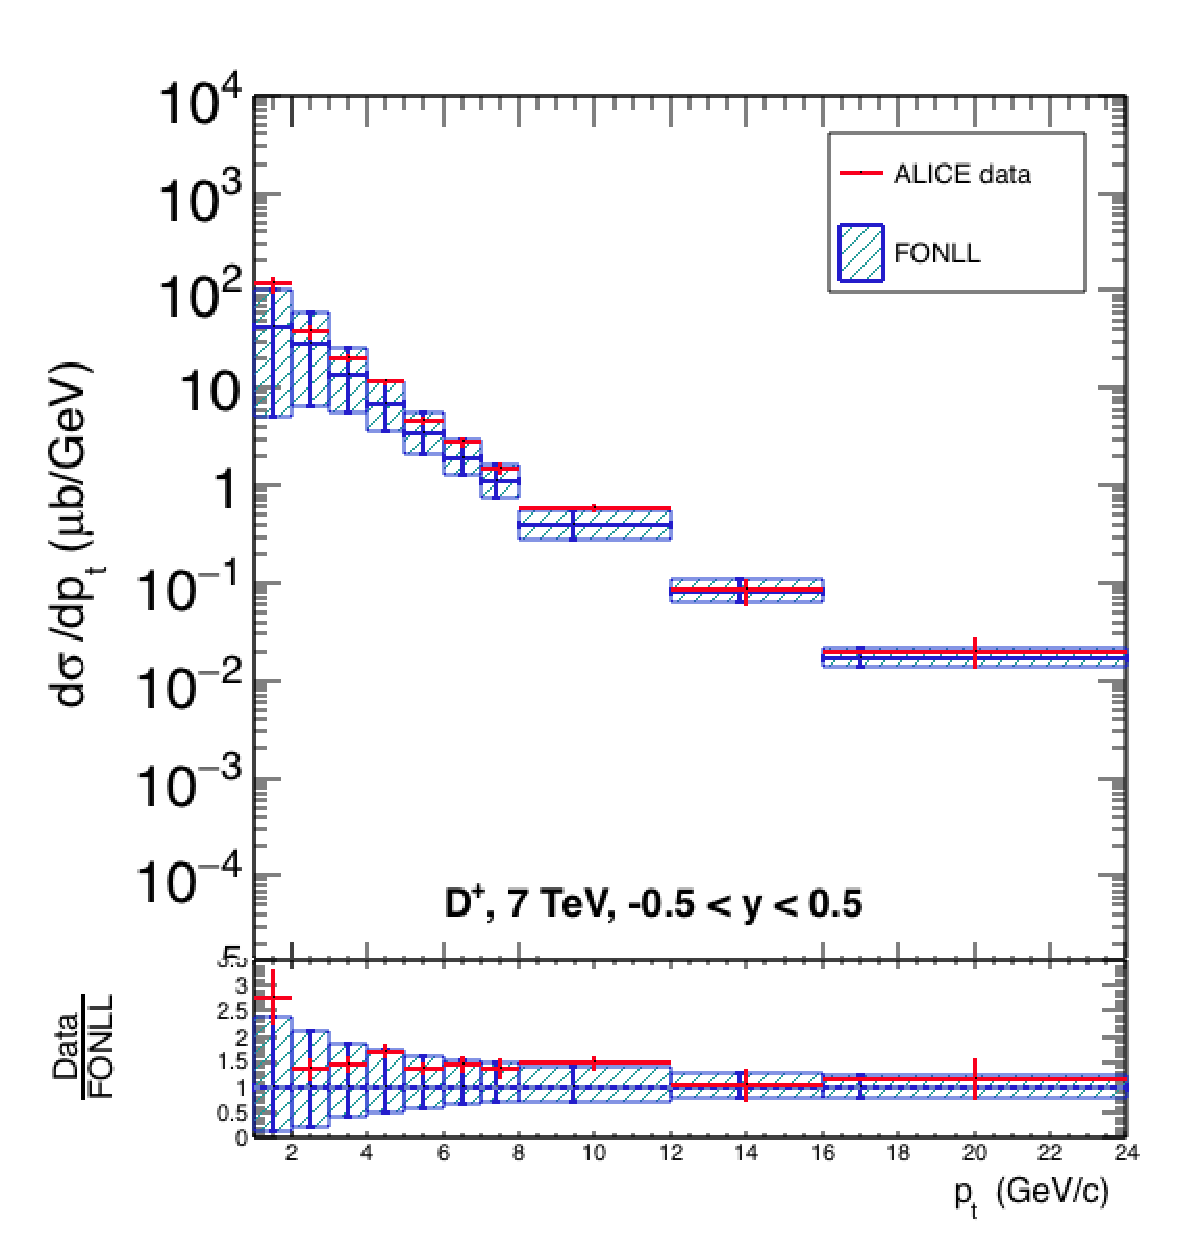
\includegraphics[width=.45\textwidth]{FigCap4/Dplus_7TeV_y_05_05.eps}
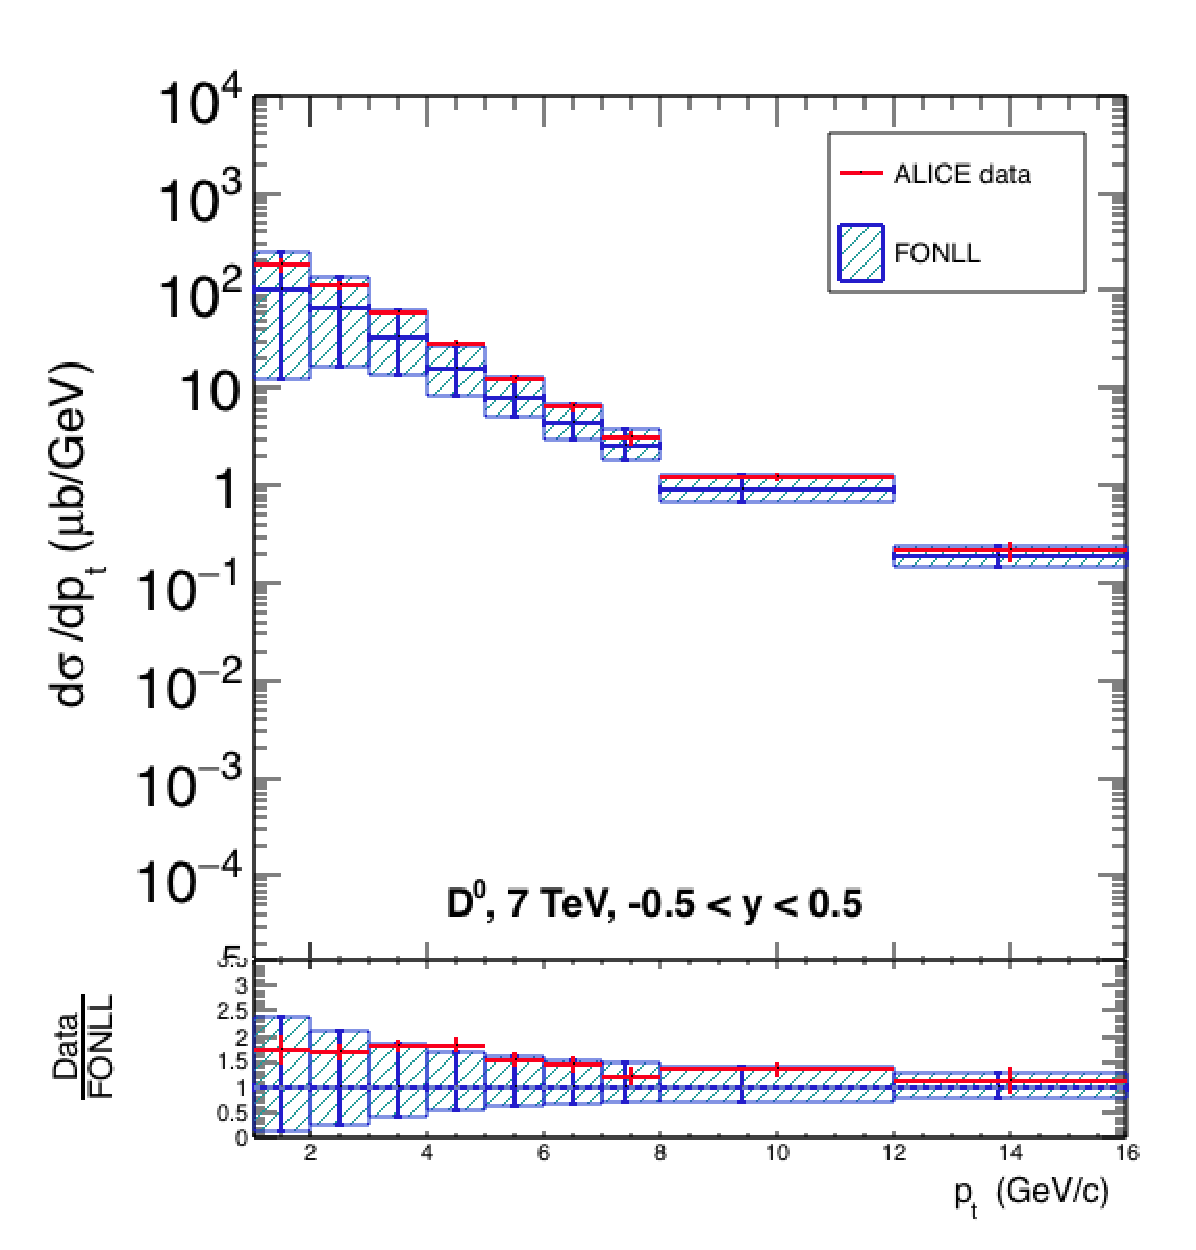
\includegraphics[width=.45\textwidth]{FigCap4/Dzero_7TeV_y_05_05.eps}
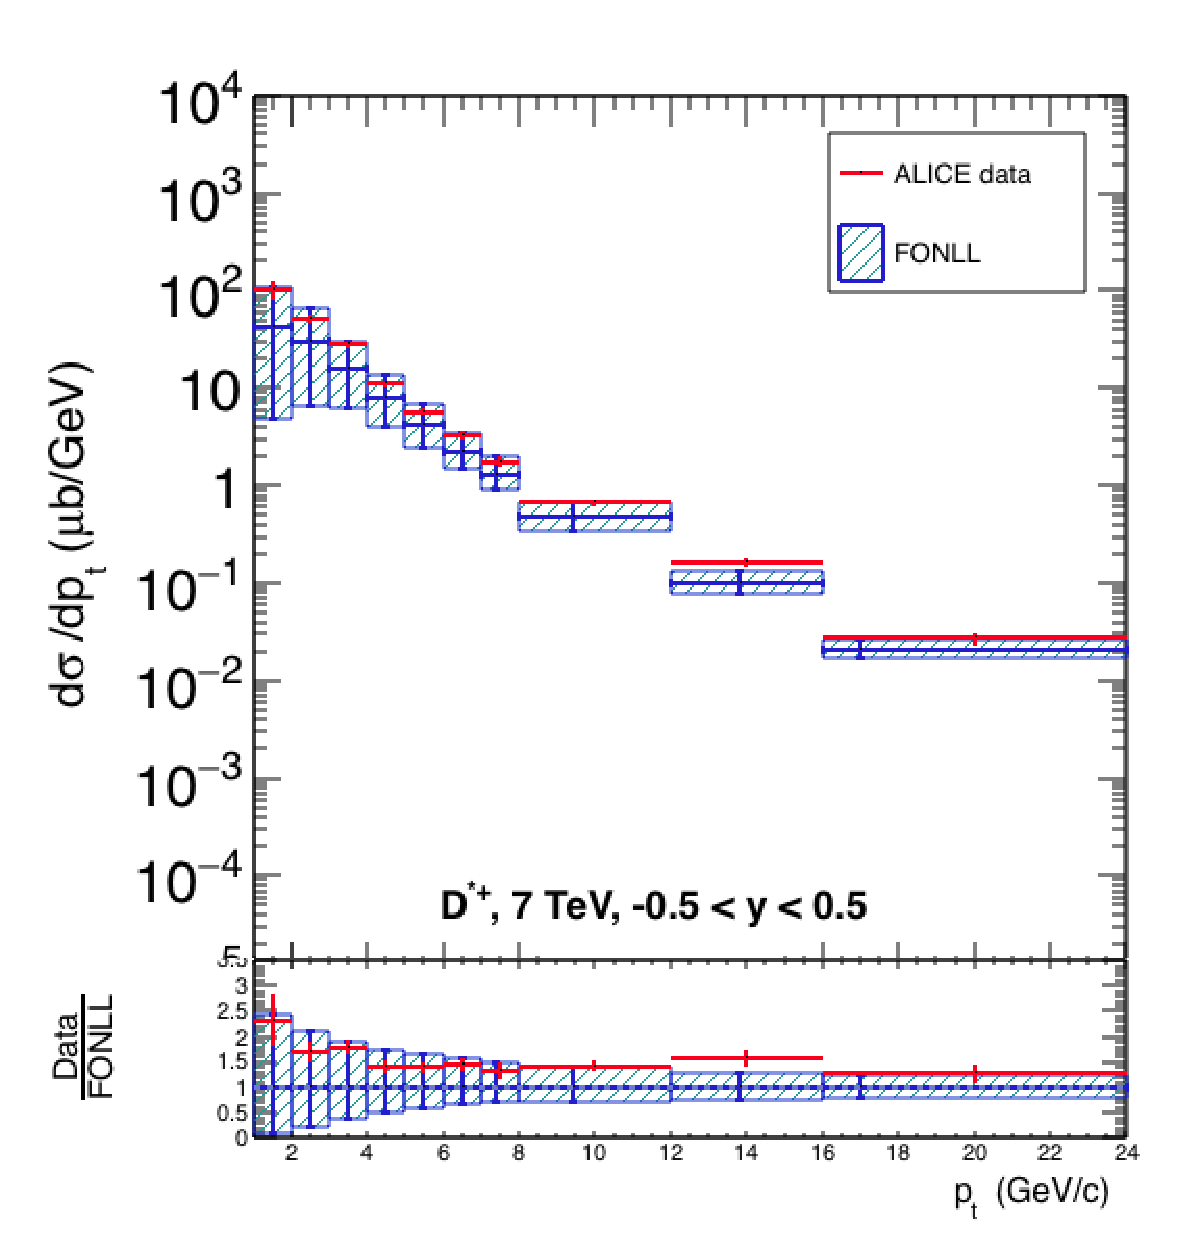
\includegraphics[width=.45\textwidth]{FigCap4/Dstar_7TeV_y_05_05.eps}
\caption{J/$\psi$ (from LHCb, \mbox{2 $< y_{cm} <$ 4.5}), D$^{+}$, D$^{0}$ and D$_{\rm s}$ (from ALICE, mid-rapidity) differential cross-sections (red points) as a function of $p_{\rm T}$ in pp collisions at 7 TeV compared with FONLL predictions at the same energy (blue boxes). }
\label{fig:Dmesons}
\end{center}
\end{figure}
